\chapter{An Algorithm for Non-Synchronizable Dynamical Systems}\label{cap:5}


{\lettrine[loversize=0.25,findent=0.2em,nindent=0em]{I}{n} this chapter we approach discrete dynamical systems that are not synchronizable. As there are no synchronization words, the methods using the ALEPH algorithm are not applicable for this category of systems. In order to model them we present another algorithm, the D-Markov Model with Graph Minimization (DMGM) algorithm. In Section \ref{sec:dmgm} we describe the DMGM algorithm step by step. In the next section, three examples of applications are shown in order to compare the results obtained by DMGM against those from a D-Markov model. The first example is of a synchronizable machine, the ternary even shift presented in Section \ref{sec:terneven}, so it is possible to see that although DMGM is not intended for this kind of application it still can produce considerably good results, although worse than those from ALEPH. We also consider two examples of non-synchronizable dynamical systems: the logistic map, which is a discrete mapping that can present chaotic behavior, and the binary communication channel with fading, that is useful for modeling wireless communications.

\section{DMGM Algorithm}\label{sec:dmgm}

D-Markov models usually achieve good performance modeling non-synchronizable dynamical systems as $D$ grows, which means that the cost for this improved performance is an exponential growth in the number of states. The DMGM algorithm comes as an improvement of D-Markov models using some graph minimization techniques presented before to reduce the size of the final machine. The full algorithm is shown in Algorithm \ref{alg:dmgm}.

The central idea of DMGM is to partition the states of the D-Markov machine into equivalence class, grouping states with statistically similar morphs together in the same class, similarly to what is done in the ALEPH algorithm. As the number of equivalence classes is usually less than the total number of states (the worst case scenario being when each state is in its own individual class), this step represents a compression, but it also makes the structure non-deterministic (i.e. a class might have transitions to more than one class with the same symbol) so some splitting is necessary to obtain a deterministic topology. 

Some states might be incorrectly grouped together as their morph might not be reliable. This happens when the probability of occurrence of a state in the original sequence is relatively low or when the input sequence is too short and statistics for longer subsequences rely on a lower count of occurrences. In order to correct these errors, a subset of the equivalence classes are split into three new classes each, depending on how the occurrence probability of each state deviates from the average occurrence probability of that class.

Once these equivalence classes are obtained, a graph minimization algorithm such as Moore or Hopcroft is applied to them in order to split equivalence classes that create a non-deterministic PFSA topology until an irreducible deterministic topology is obtained for the PFSA. This PFSA is then output as the final result of the algorithm.

Each step of this algorithm is discussed in more details in the following sections.

\subsubsection{Step 1: Create D-Markov Machine}

DMGM starts by creating a D-Markov model $\mathcal{D}$ for an input $D$ and the original sequence $S$ value which should have its number of states reduced in the following steps.

\subsubsection{Step 2: Group states together in equivalence classes}

This step starts by creating an initial equivalence class $P_0$ containing a state from $\mathcal{D}$ and the list $\mathcal{P}$ of equivalence classes is initialized containing $P_0$. The algorithm then checks the remaining states of $\mathcal{D}$ using the same criterion used in ALEPH: if a state $s$ from $\mathcal{D}$ and $P[0]$, which is the first state in the equivalence class $P$ for some $P\in\mathcal{P}$, pass in a statistical test performed by the auxiliary function \textit{statisticalTest}($p, q, \alpha$), which compares the morph of $p$ to the morph of $q$ using a statistical test (either $\chi^2$ or Kolmogorov-Smirnov) with confidence level $\alpha$, $s$ is added to the equivalence class $P$. If $s$ passes in no tests, a new equivalence class $R$ is created containing only $s$ and $R$ is added to $\mathcal{P}$.

\subsubsection{Step 3: Compute averages and standard deviations}

The next step consists of computing the average and standard deviation of the occurrence probability for each equivalence class. This means that, for each class, there is a probability of occurrence for each state in it, i.e. the probability that the state's label occurs in the original sequence. These information should be stored after computing the transition probabilities of $\mathcal{D}$. For each class $P\in\mathcal{P}$, the average probability of occurrence is computed with the auxiliary function \textit{average}($P$) and it is stored in \textit{avgs}$_P$. Similarly, the standard deviation is calculated by the auxiliary function \textit{std}($P$) and it is stored in \textit{stds}$_P$.

\subsubsection{Step 4: Split the classes with highest standard deviations}

Let $H$ be the number of equivalence classes with the highest standard deviation. These classes are stored in \textit{hi-stds} to be split in new equivalence classes. This is done because although the states in these classes have similar morphs, the ones that diverge significantly from the average for the class (i.e. are $t$ standard deviations away from the average) might not have reliable morphs and should be grouped in a different equivalence class. This might happen when a state is relatively rare compared to the others or if the input sequence is not long enough and the statistics of longer states can not be considered reliable.

The classes of \textit{hi-stds} should be removed from $\mathcal{P}$. And then, for each class $E \in$ \textit{hi-stds}, the equivalence classes \textit{hi}, \textit{lo} and \textit{mid} are initialized empty and then for each state $e \in E$, it is checked if $\Pr(e)$ (the probability of occurrence of $e$) is greater than \textit{avgs}$_e + t\cdot$ \textit{stds}$_E$ (greater than $t$ standard deviations above the average). If it is, $e$ is grouped in \textit{hi}. If not, it is checked if it is lesser than \textit{avgs}$_E - t\cdot $ \textit{stds}$_E$ (lesser than $t$ standard deviations below the average) and in the affirmative case it is grouped in \textit{lo}. If none of the above conditions is met, $e$ is grouped in $mid$. After each state of $E$ is either in \textit{hi}, \textit{lo} or \textit{mid}, these three equivalence classes are appended to $\mathcal{P}$.

\subsubsection{Step 5: Apply graph minimization algorithm}

The final step consists of applying a graph minimization algorithm (either Moore or Hopcroft) to this final set of equivalence classes. The resulting PFSA is capable of achieving a performance close to the original D-Markov machine while reducing its number of states. 

  \begin{algorithm}[H]
  \caption{DMGM($S, D, H, t, \alpha$)\label{alg:dmgm}}
    \begin{algorithmic}[1]
      \Procedure{DMGM}{}
      	\State \textbf{\#\# Step 1: Create D-Markov Machine}
      	\State $\mathcal{D} \gets$ \textit{dmarkov}($S,D$)
      	\State \textbf{\#\# Step 2: Group states together in equivalence classes}  
      	\State $P_0 \gets \{$ any state from $\mathcal{D}\}$    	
      	\State $\mathcal{P} \gets \{P_0\}$
      	\For{$s \in \mathcal{D}$}
      		\For{$P \in \mathcal{P}$}
      			\State $r \gets$ \textit{statisticalTest}($s, P[0], \alpha$)
      			\If{$r =$ True}
      				\State $P \gets P \cup \{s\}$
      			\Else
      				\State $R \gets \{s\}$
      				\State $\mathcal{P} \gets \mathcal{P}\cup R$
      			\EndIf
      		\EndFor
      	\EndFor
      	\State \textbf{\#\# Step 3: Compute averages and standard deviations}
      	\For{$P \in \mathcal{P}$}
      		\State \textit{avgs}$_P \gets$ \textit{average}($P$)
      		\State \textit{stds}$_P \gets$ \textit{std}($P$)
      	\EndFor      	
      	\State \textbf{\#\# Step 4: Split the classes with highest standard deviations}
      	\State \textit{hi-stds} $\gets$ the $H$ classes in $\mathcal{P}$ with the highest \textit{stds}values
      	\State Remove the classes in \textit{hi-stds} from $\mathcal{P}$
      	\For{$E \in$ \textit{hi-stds}}
      	    \State \textit{\#\# hi, mid and lo are initialized as empty lists}
      		\State \textit{hi}, \textit{mid}, \textit{lo}$ \gets \emptyset$
      		\For{$e \in E$}
      			\If{$\Pr(e) \geq$ \textit{avgs}$_E+ t\cdot $ \textit{stds}$_E$}
      				\State \textit{hi} $\gets$ \textit{hi} $\cup \{e\}$
      			\ElsIf{$\Pr(e) \leq $ \textit{avgs}$_E+ t\cdot $ \textit{stds}$_E$}
      				\State \textit{lo} $\gets$ \textit{lo} $\cup \{e\}$
      			\Else      				
      				\State \textit{mid} $\gets$ \textit{mid} $\cup \{e\}$
      			\EndIf
      		\EndFor
      		\State $\mathcal{P} \gets \mathcal{P}\cup\{$ \textit{hi, lo, mid} $\}$
      	\EndFor
      	\State \textbf{\#\# Step 5: Apply graph minimization algorithm}
      	\State $G \gets$ \textit{graphMinimization}($\mathcal{P}$)
      	\State \textbf{return} $G$
      \EndProcedure
    \end{algorithmic}
  \end{algorithm}
  
\subsection{Time Complexity}

Generating the D-Markov machine from the original sequence $S$ of length $N$ has a complexity of $O(N)$.The main component of the complexity of DMGM is the partitioning into equivalence classes. As in ALEPH, this step requires visiting each state and comparing it to the current equivalence classes, which for a D-Markov machine with $D$ states and over an alphabet $\Sigma$ takes $O(|\Sigma|^D)$. 

Steps 3 and 4 operate over a subset of equivalence classes of size $H$ which might contain at most $\xi \leq |\Sigma|^D$ states (with equality holding when $H$ is equivalent to the total number of equivalence classes). In these steps, each of the $\xi$ states is visited in order to split them into three new equivalence classes. This takes at most $O(\xi)$ and it can be safely be ignored from the final complexity.

Finally, the graph minimization algorithm checks all states in the equivalence classes again so they can be split appropriately (as in the Moore algorithm), therefore its complexity multiplies the complexity of Step 2 by $O(|\Sigma|^D)$. This gives DMGM a final complexity of $O(N + |\Sigma|^{2D})$. If the sequence is larger than the square of the number of states in the D-Markov machine, it dominates the complexity. Otherwise, the partitioning in equivalence classes is the biggest part.

Although DMGM is necessarily more complex as D-Markov (as one of its steps includes generating a D-Markov machine), it is shown in the next section that its final results are considerably more compact than those from D-Markov machines. Generating the PFSA is a one-time endeavor, while using it in its applications is probably done more frequently, which means it compensates to have a smaller PFSA even if it takes a little longer to obtain it. 

\section{Applications}

In this section, three examples of applications of the DMGM algorithm are shown. First, DMGM is applied to the ternary even shift, that was previously covered in Section \ref{sec:terneven} and is a synchronizable system. This is done in order to verify how it behaves when applied to a category of systems for which it is not designed. The two other examples are non-synchronizable systems: the logistic map, which can show chaotic behavior, and the binary fading channel, which is an important system to simulate wireless communication systems.  The values of $H$ and $t$ used in each case were obtained by trial and error to obtain the best results, as there is still not a method to compute their optimum value for these parameters.

\subsection{Ternary Even Shift}

As seen in Section \ref{sec:terneven}, the ternary even shift is a synchronizable dynamical system with three states over a ternary alphabet. When the ALEPH algorithm is applied to a sequence $S$ of length $10^7$ generated by the ternary even shift, it is capable of recovering the original PFSA.

When DMGM is applied to $S$, its results for conditional entropy and Kullback-Leibler divergence vs. number of states using $\ell=10$, $\alpha = 0.95$, the $\chi^2$ test and DMGM parameters $H=1$ and $t=1$ for $D$ from 2 to 10 are shown in Figures \ref{fig:ternevenhdmgm} and \ref{fig:ternevenklddmgm}, respectively. Although DMGM is not capable of retrieving the original machine as ALEPH, for $D = 8$ it is possible to see that it creates a machine that performs similarly to the original with 17 states and the correspondent D-Markov machine has 681. The DMGM is not significantly larger than the original three state machine and still has a smaller size compared to the D-Markov machine.

In fact, it is observed that for any $D$, the machine obtained by DMGM is much more compact than the correspondent D-Markov machine. For $D=2$ the difference is of $44.4\%$ while for $D = 10$ it reaches $99.2\%$. This shows that although DMGM is not optimal for synchronizable systems, its results are still considerably good in these cases. When it is uncertain if the system to be modeled is synchronizable or not it might be a good idea to apply DMGM as it probably can achieve good results.

\begin{figure}[h]
\centering
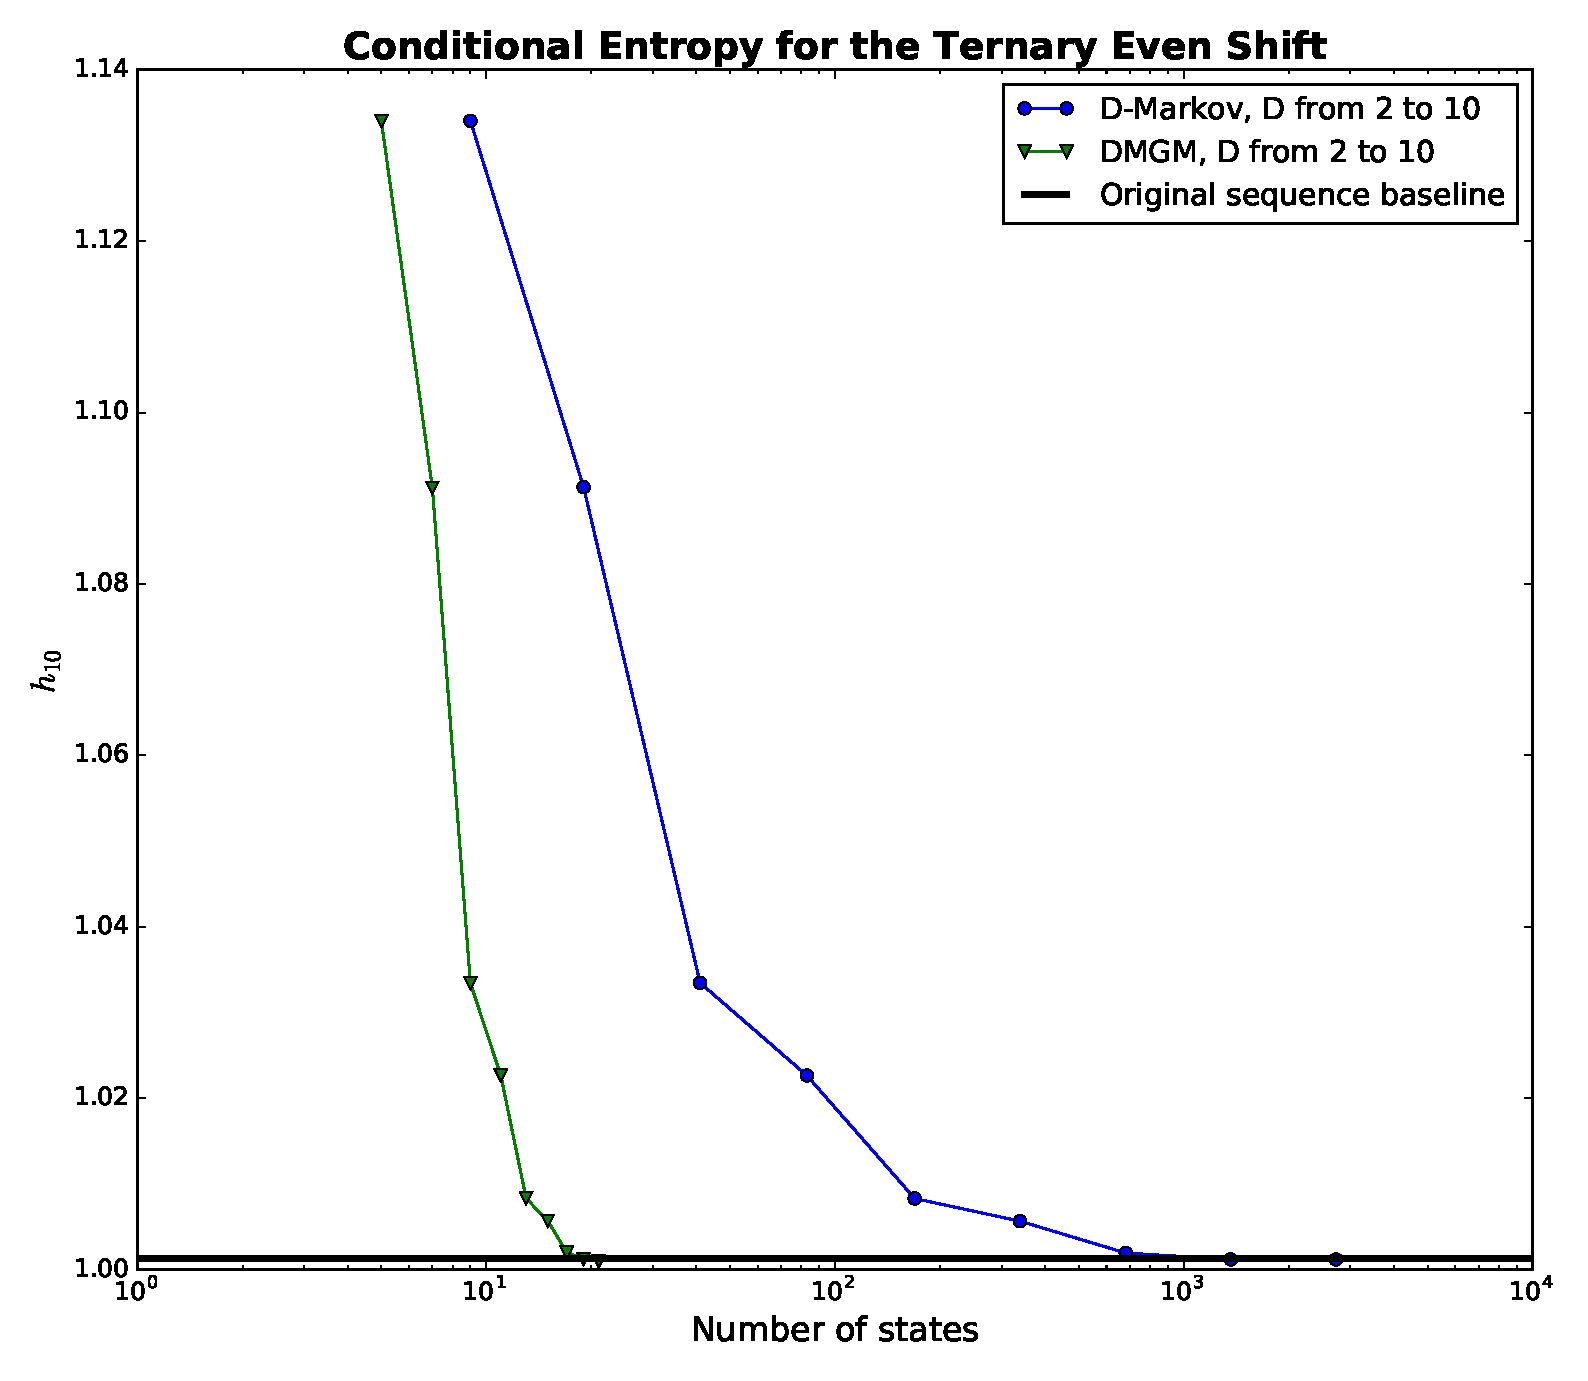
\includegraphics[scale=0.35]{Figuras/ternaryeven_h_mk4.eps}
\caption{Conditional entropy $h_{10}$ of sequences generated by D-Markov machines and DMGM PFSA by the number of states of the machine that generated them, with $D$ ranging from 2 to 10, $H=1$ and $t=1$ for the ternary even shift.\label{fig:ternevenhdmgm}}
\end{figure}

\begin{figure}[h]
\centering
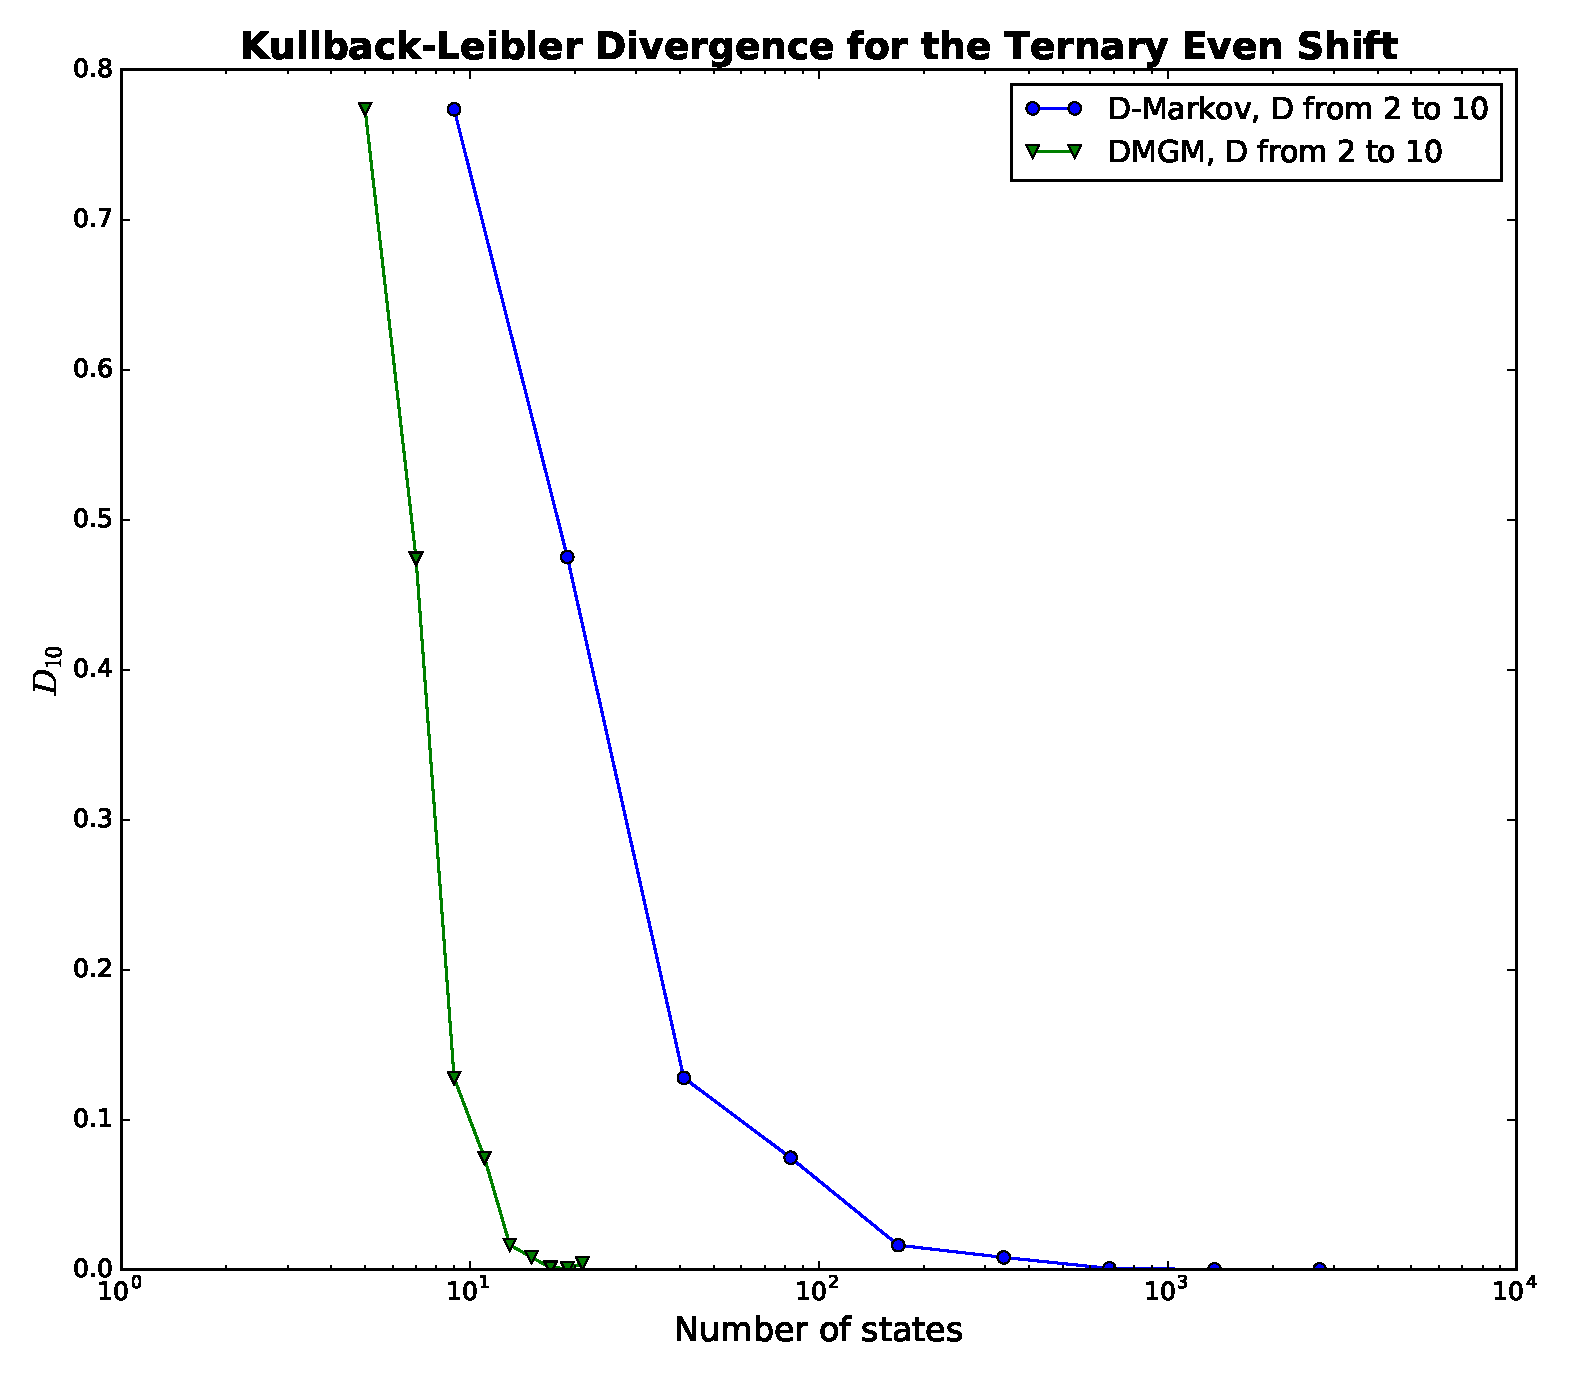
\includegraphics[scale=0.35]{Figuras/ternaryeven_kld_mk4.eps}
\caption{Kullback-Leibler divergence $D_{10}$ versus the number of states of sequences generated by D-Markov machines and DMGM PFSA compared to the original sequence $S$, with $D$ ranging from 2 to 10, $H=1$ and $t=1$ for the ternary even shift.\label{fig:ternevenklddmgm}}
\end{figure}


\FloatBarrier

\subsection{Logistic Map}

%The next two examples show how the algorithms fare when modeling a system whose PFSA is unknown or non-existent. A sequence from these systems will be analyzed and a PFSA model will be created and its output will be compared to the original sequence to see how well this Markovian model approximates a dynamic system which might not even be Markovian.

The first of example of non-synchronizable dynamical system is the Logistic Map, a symbolic dynamic system whose outputs are given by the difference equation \cite{strogatz2001nonlinear}:

\begin{equation}
x_{k+1} \triangleq rx_k(1-x_k), \label{eq:logisticmap}
\end{equation}


\noindent which shows chaotic behavior for several values of $r$. As in \cite{asok.14}, $x_0$ is set to $0.5$ and $r = 3.75$. A sequence of length $10^7$ is generated from this equation and then it is quantized with a ternary alphabet: values $x_k \leq 0.67$ are mapped to $0$; when $0.67 < x_k \leq 0.79$, it is mapped to 1 and when $x_k > 0.79$ it is mapped to $2$. A part of that sequence and the specified threshold are shown in Figure \ref{fig:lmapseq}.

\begin{figure}[b]
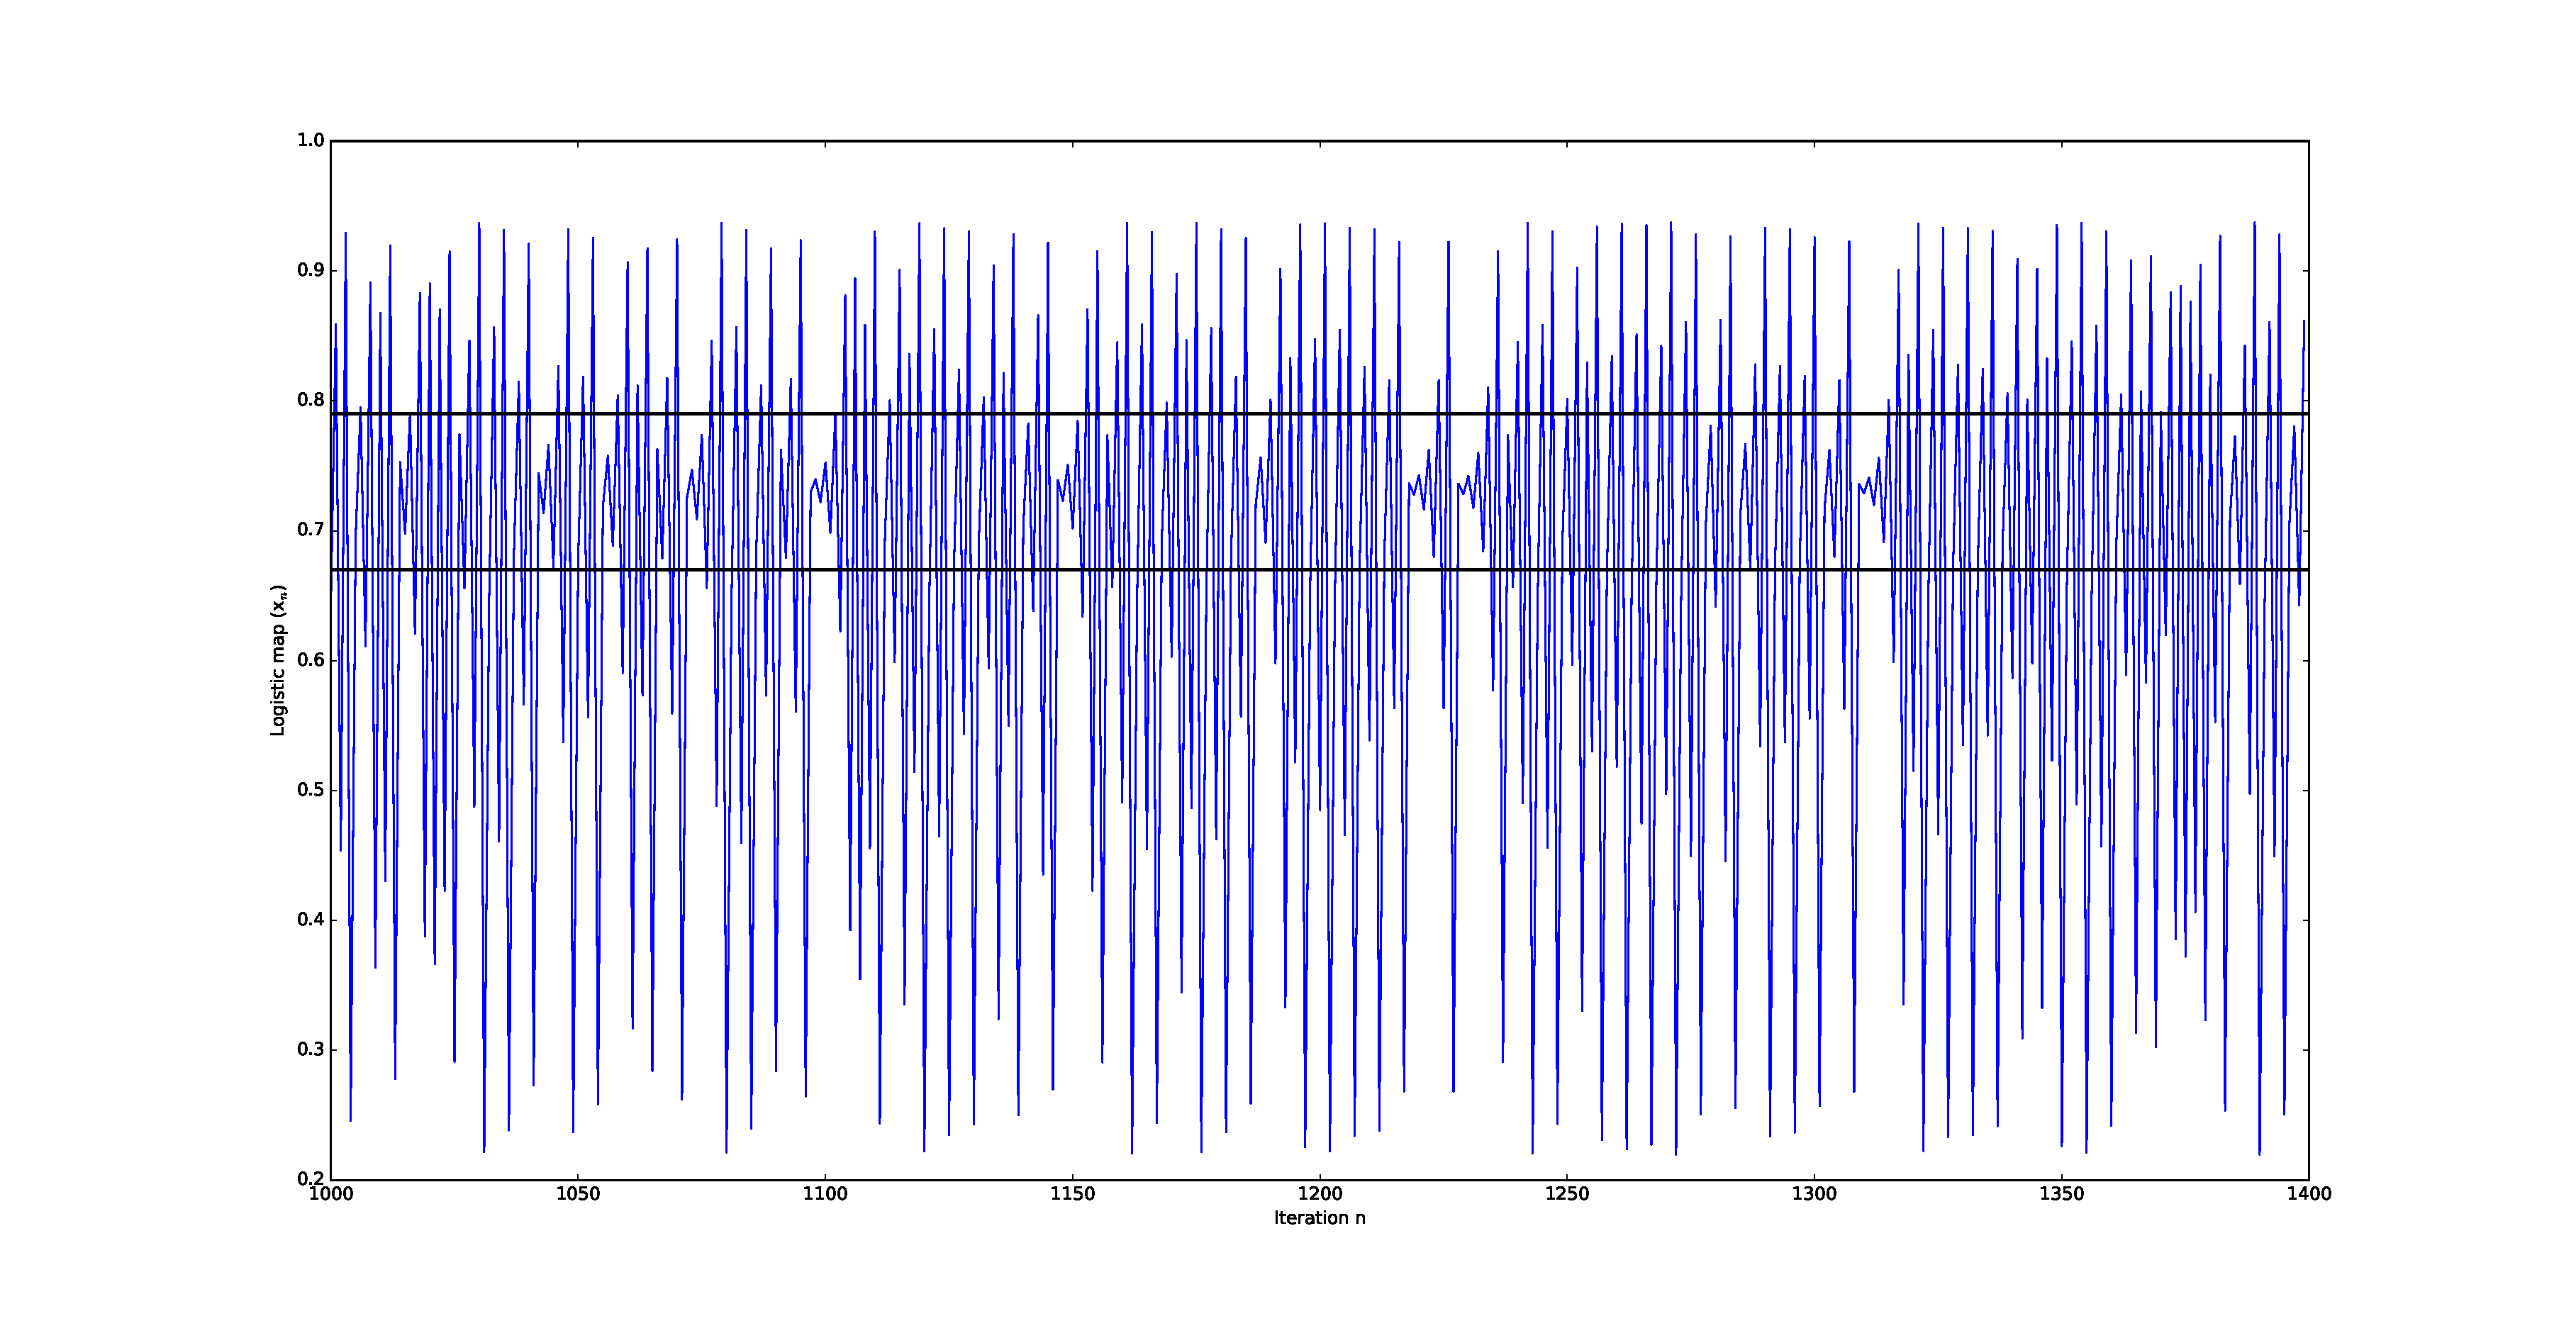
\includegraphics[scale=0.25]{Figuras/logisticmap.eps}
\caption{Samples of the Logistic Map sequence generated by (\ref{eq:logisticmap}) with $x_0$ = 0.5 and $r$ = 3.75.\label{fig:lmapseq}}
\end{figure}

D-Markov machines were generated from the ternary sequence $S$ for $D$ from 4 to 12 and they were used as basis for DMGM machines for the same range. The comparative results for conditional entropy  for $\ell = 10$ versus the number of states are shown in Figure \ref{fig:lmapent} and the results for Kullback-Leibler divergence for $\ell = 10$ versus number of states are shown in Figure \ref{fig:lmapkld}. For these results, the value of $\alpha$ is 0.95, the statistical test is $\chi^2$ test and the parameters for DMGM are $H = 3$ and $t = 1$ . Each mark in the curves of Figures \ref{fig:lmapkld} and \ref{fig:lmapent} indicate one machine, starting with $D=4$ in the upper left.

\begin{figure}[h]
\centering
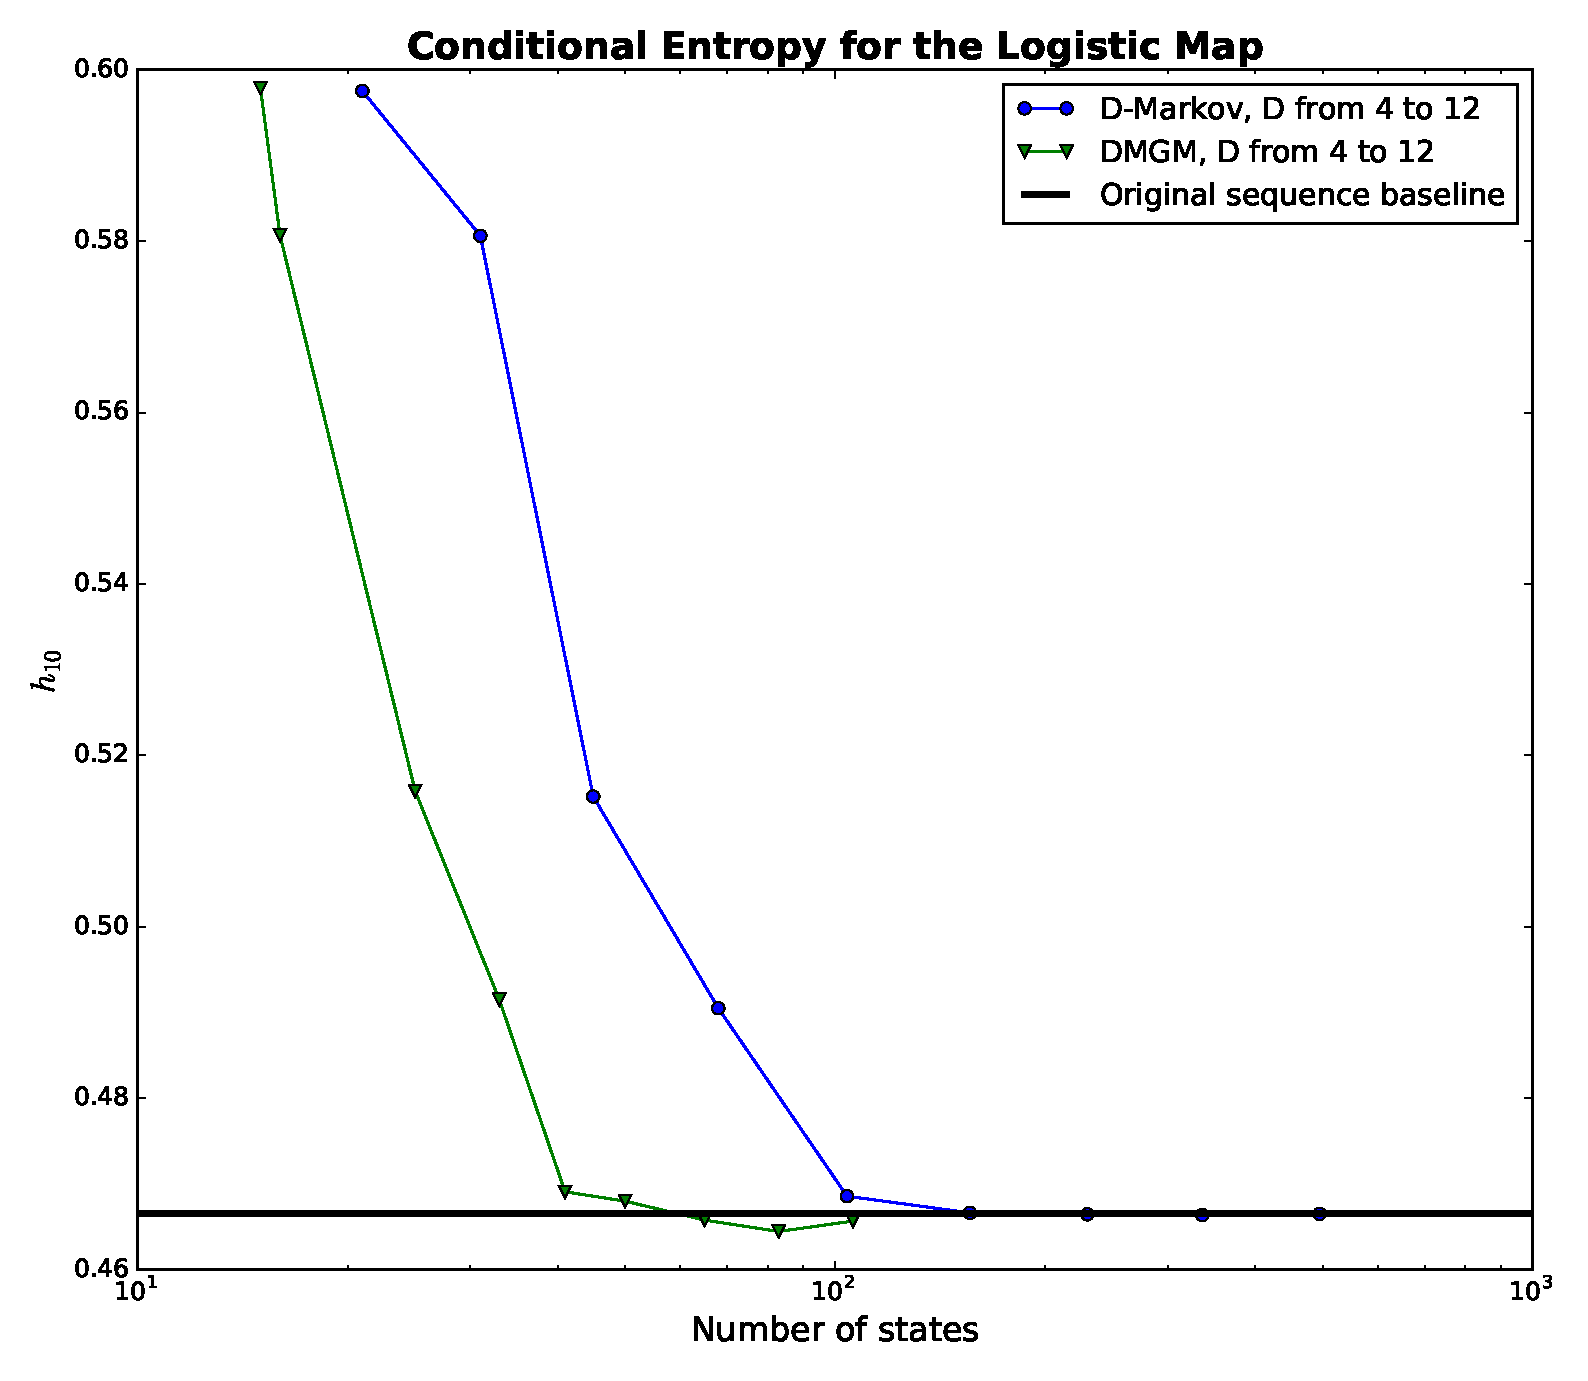
\includegraphics[scale=0.35]{Figuras/logisticmap_h_mk4.eps}
\caption{Conditional entropy $h_{10}$ versus the number of states of sequences generated by D-Markov machines and DMGM PFSA with $D$ ranging from 4 to 12, $H=3$ and $t=1$ for the logistic map.\label{fig:lmapent}}
\end{figure}

\begin{figure}[h]
\centering
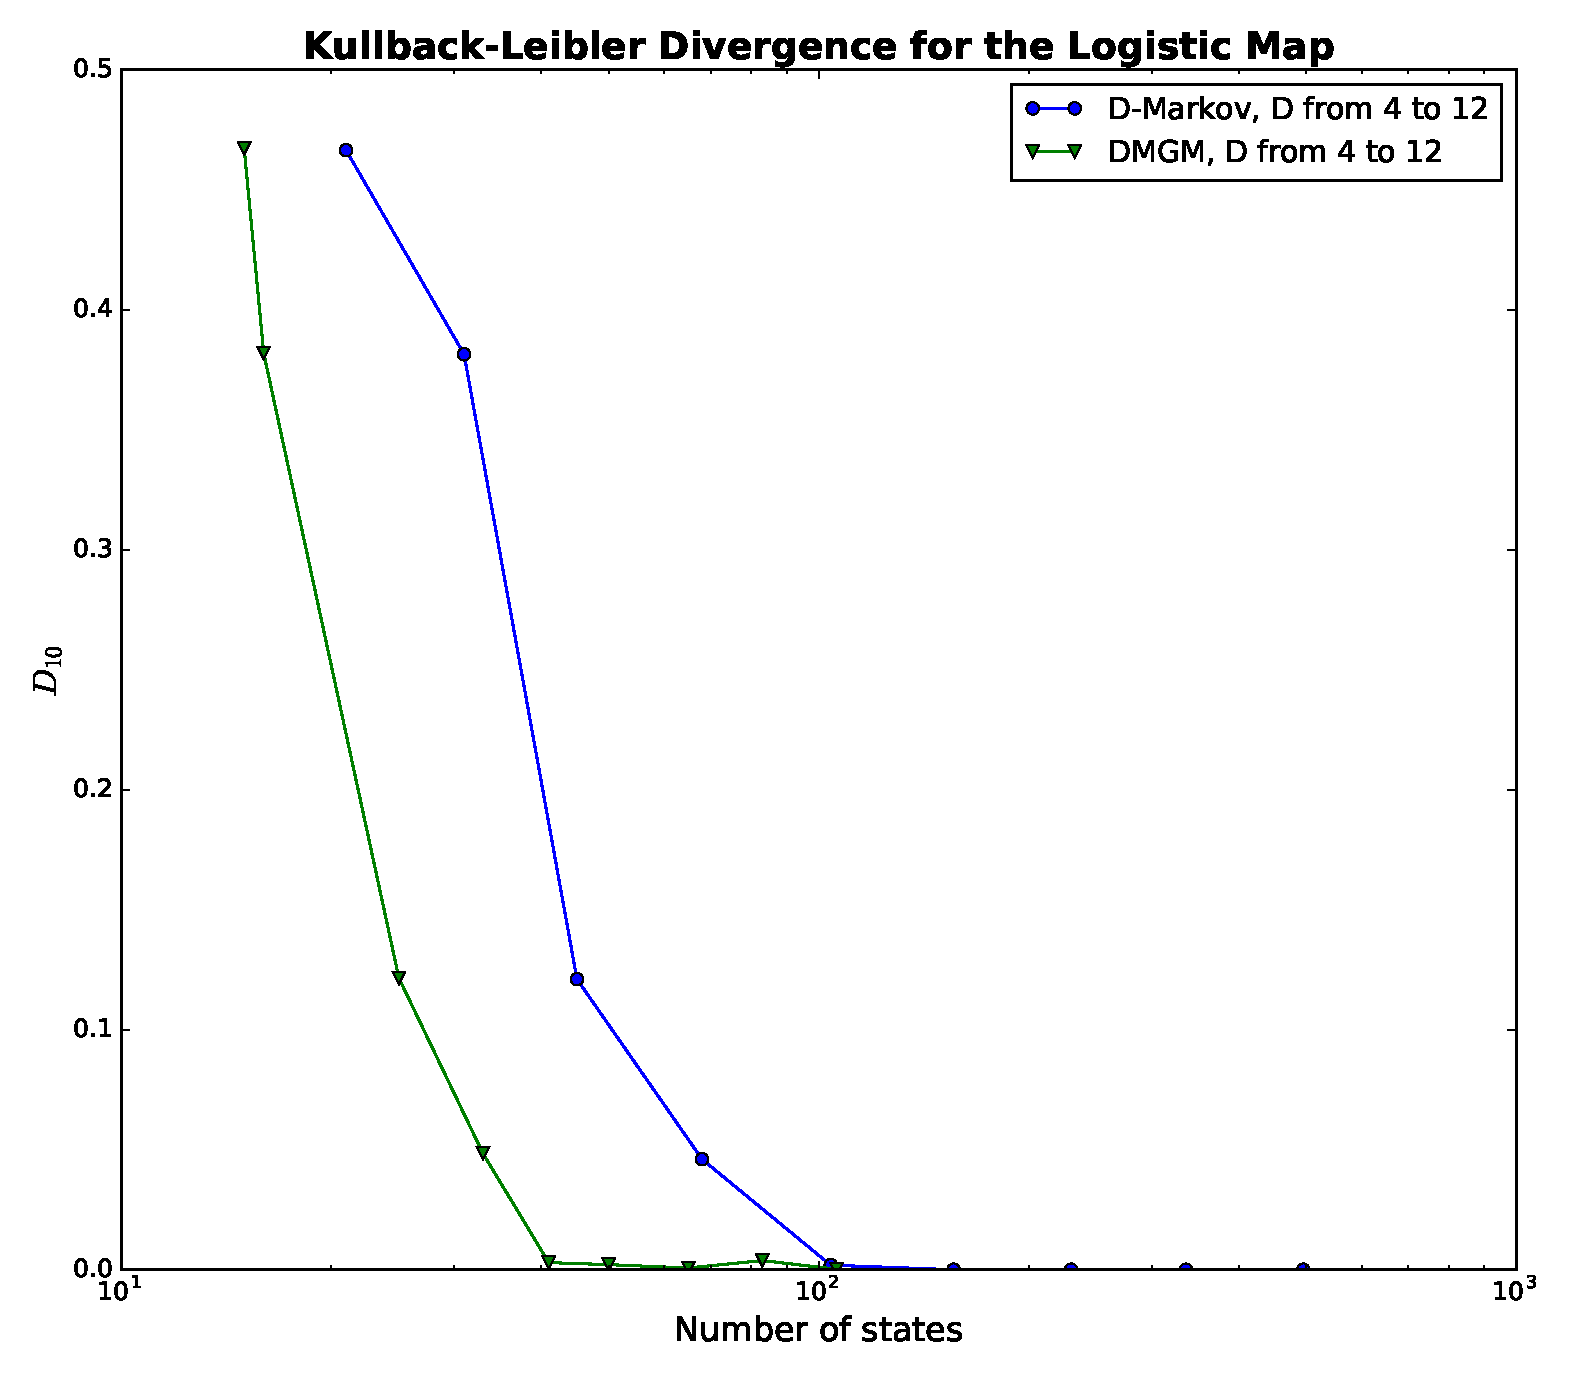
\includegraphics[scale=0.35]{Figuras/logisticmap_kld_mk4.eps}
\caption{Kullback-Leibler divergence $D_{10}$ versus the number of states of sequences generated by D-Markov machines and DMGM PFSA compared to the original sequence $S$ with $D$ ranging from 4 to 12, $H=3$ and $t=1$ for the logistic map.\label{fig:lmapkld}}
\end{figure}

As the scale of the x-axis is logarithmic it is possible to see that the states of both D-Markov machines and DMGM PFSA grow exponentially with $D$, although the number of states of DMGM grows slower than the D-Markov machines. For a given $D$ it is possible to see that the quality of the D-Markov machine and of the DMGM PFSA are similar, indicating that the DMGM machine is a more suitable candidate to model the original system as it is more compact while performing similarly to the D-Markov machines.  This is observed by noting that for $D = 4$, DMGM is capable of obtaining a machine $28.6\%$ smaller than D-Markov, while for $D = 8$, DMGM is $60.6\%$ more compact than the respective D-Markov machine. 

%From these figures it is possible to see that the performance of a DMGM is similar to the correspondent D-Markov machine for a given $D$ but with a reduced numbered of states. Also, as $D$ increases, the performance also increases, but the number of states does not grow as fast as the number of states of the D-Markov machine, showing that the DMGM is a good algorithm to create models for the logistic map.

In Figure \ref{fig:lmapent}, it is shown that for $D = 8$ both types of machines are capable of capturing the original system memory, but DMGM achieves this with 41states, while D-Markov needs 104 states. Similarly, in Figure \ref{fig:lmapkld}, the divergence of machines with $D \geq 8$ in relation to the original becomes sufficiently close to zero, which means they are able to generate sequences similar to the original system. Using $D < 8$ might be useful to obtain more compact models, in expanse of them being less precise. 



\FloatBarrier
\subsection{Binary Fading Channel}

Consider a binary-input binary-output discrete fading channel (DFC) with a binary input process $\{X_k\}_{k=1}^{\infty}$, $X_k \in \{0,1\}$, 
and a binary output process $\{Y_k\}_{k=1}^{\infty}$,  $Y_k \in \{0,1\}$.

The DFC is composed of a BPSK modulator,
a time-correlated flat Rayleigh fading channel with AWGN, and a hard-quantized 
coherent demodulator.  The  received symbol 
 at the $k$th signaling interval 
is written as
\begin{equation*}
R_k = \sqrt{E_s} A_k S_k \, + \, N_k, \quad \quad  k=1,2,\cdots
\end{equation*}
where $\{S_k\} = \{(2 X_k -1)\}$, $E_s$ is the energy of the transmitted 
signal, $\{N_k\}$ is a sequence of independent and 
identically distributed zero-mean Gaussian random variables with variance $N_0/2$. The signal to noise ratio (SNR) is defined as $E_s/N_0$
Furthermore, $\{A_k\}$ is the channel's fading process
with $A_k=|G_k|$, where $\{G_k\}$ is a complex Gaussian process with zero-mean, unit variance and Clarke's ACF~\cite{clarke1968statistical} 
$R[k] = J_0( 2 \pi f_D T |k|)$, where $J_0(x)$ is the zero-order Bessel function of the 
first kind and $f_D T$ is the normalized  maximum Doppler frequency. 
The random variable $A_k$ has the Rayleigh probability density function with unit second moment, 
$p_A(a)= 2ae^{-a^2},$ for $a >0$.
The output symbol is $Y_k=0$ if $R_k\leq 0$, or  $Y_k=1$ if $R_k > 0$.

The input and output symbols explicitly expressed in terms 
of  a noise symbol $Z_k \in \{0,1\}$ as $Y_k=X_k\oplus Z_k$, where $\oplus$ denotes addition modulo 2 and the input and noise symbols are statistically independent.
For a given DFC specified by its parameters $f_D T$, SNR, a binary noise sequence  $\{Z_k\}$ of the DFC of length $N = 3 \times 10^7$ is generated by computer simulation and the parameters of the DMGM are estimated using the algorithm proposed in the previous section.

The following results are for DMGM applied to a sequence $S$ from a binary fading channel of length $N = 3\cdot 10^7$ with $D$ varying from 4 to 9, $H= 1$, $t= 1$, $\alpha = 0.95$. Figure \ref{fig:10dbq1h} shows the result of conditional entropy versus the number of states for $\ell = 10$ and Figure \ref{fig:10dbq1kld} shows the result for Kullback-Leibler divergence versus the number of states for $\ell = 10$.

Although these results are not as significant as the ones for the logistic map, it is possible to see that DMGM still manages to produce machines that are capable of creating a machine that behaves similarly to the original system for $D=9$, for which DMGM generates a machine with 331 states and D-Markov creates one with 512 states. Also, as $D$ increases, the difference between number of states of D-Markov machines and DMGM machines increases. For $D=4$ the machines have the same number of states, while $D=9$ manages to get a difference of $35.4\%$. The only exception is for $D=6$ for which the difference does not grow significantly. 

\begin{figure}[h]
\centering
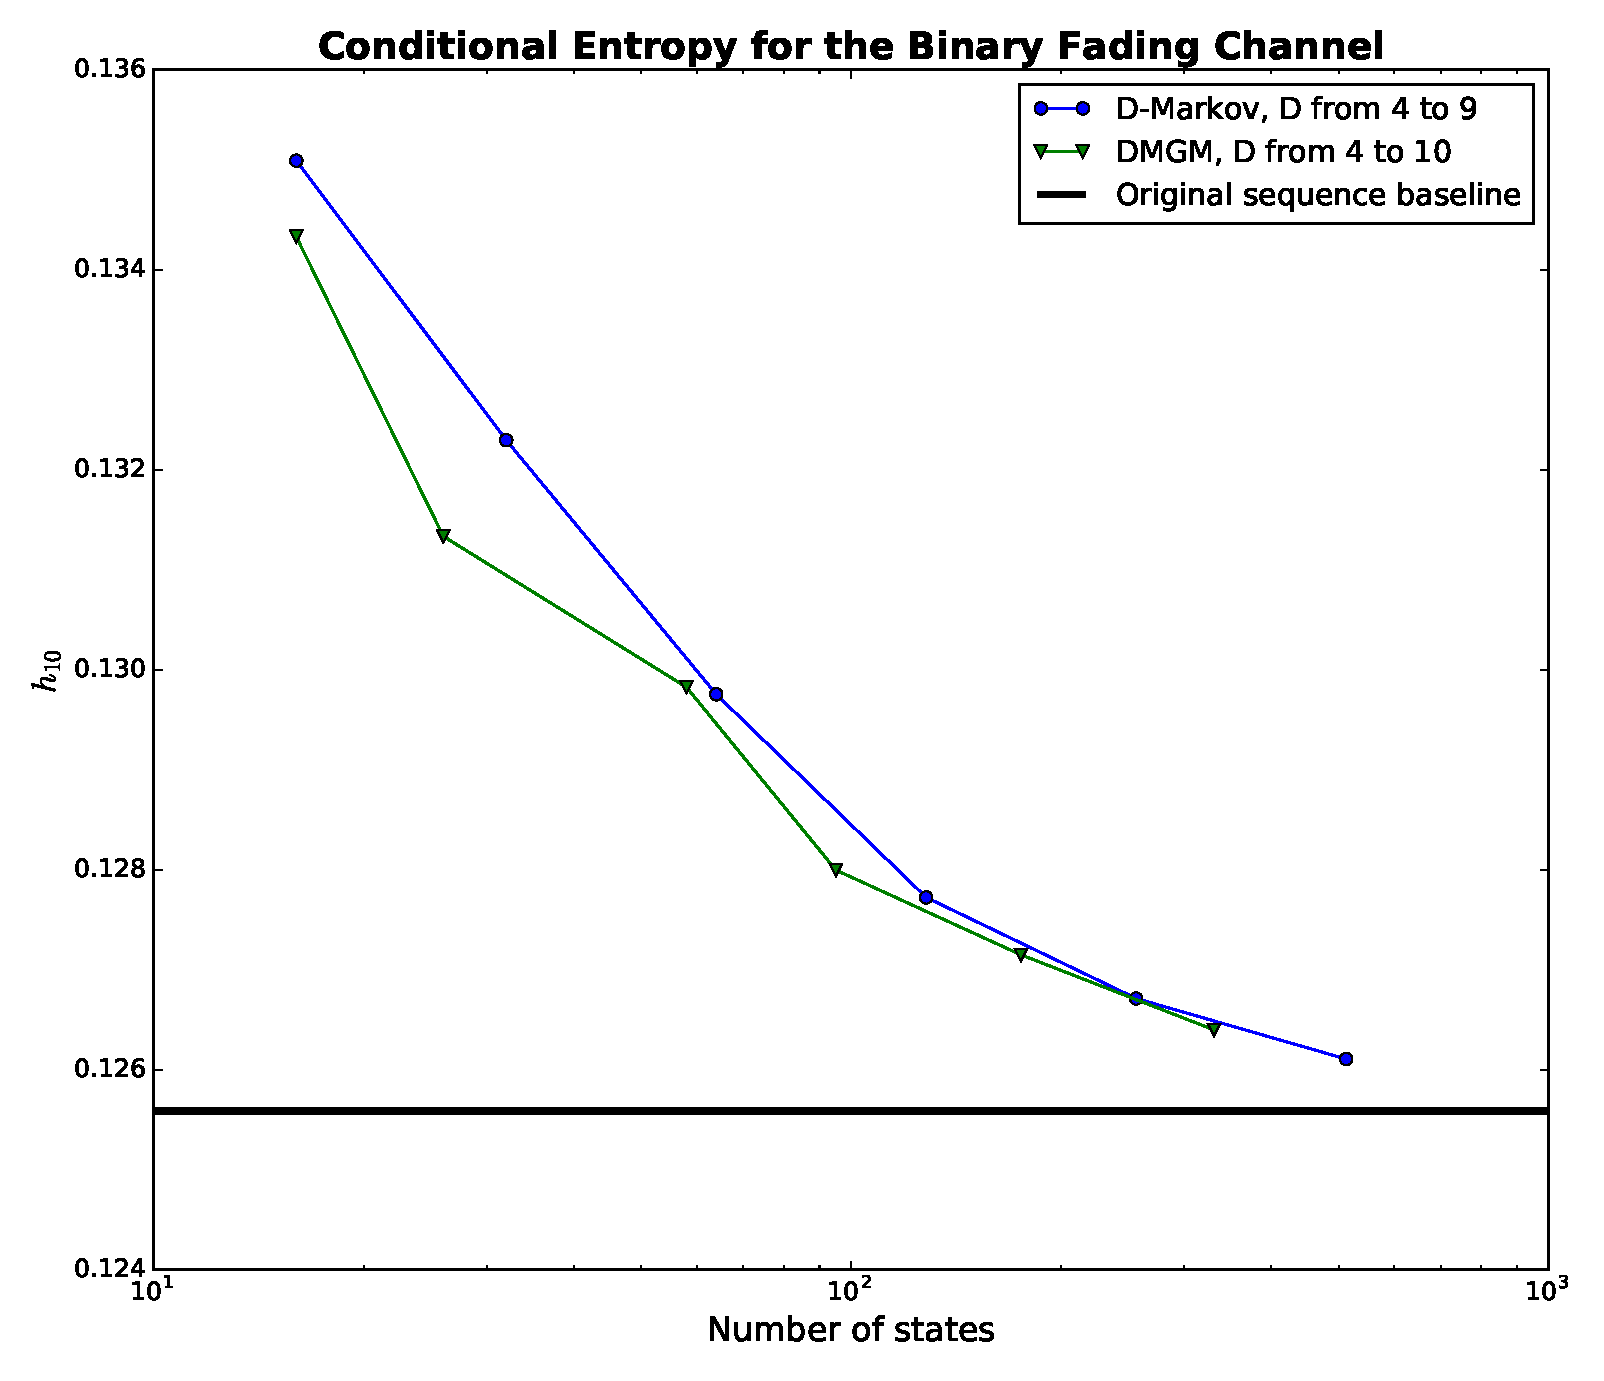
\includegraphics[scale=0.35]{Figuras/10dbq1_h_mk4.eps}
\caption{Conditional entropy $h_{10}$ of sequences generated by D-Markov machines and DMGM PFSA by the number of states of the machine that generated them, with $D$ ranging from 2 to 10, $H=1$ and $t=1$ for the binary fading channel with $f_DT = 0.05$ and $SNR = 10$dB.\label{fig:10dbq1h}}
\end{figure}

\begin{figure}[h]
\centering
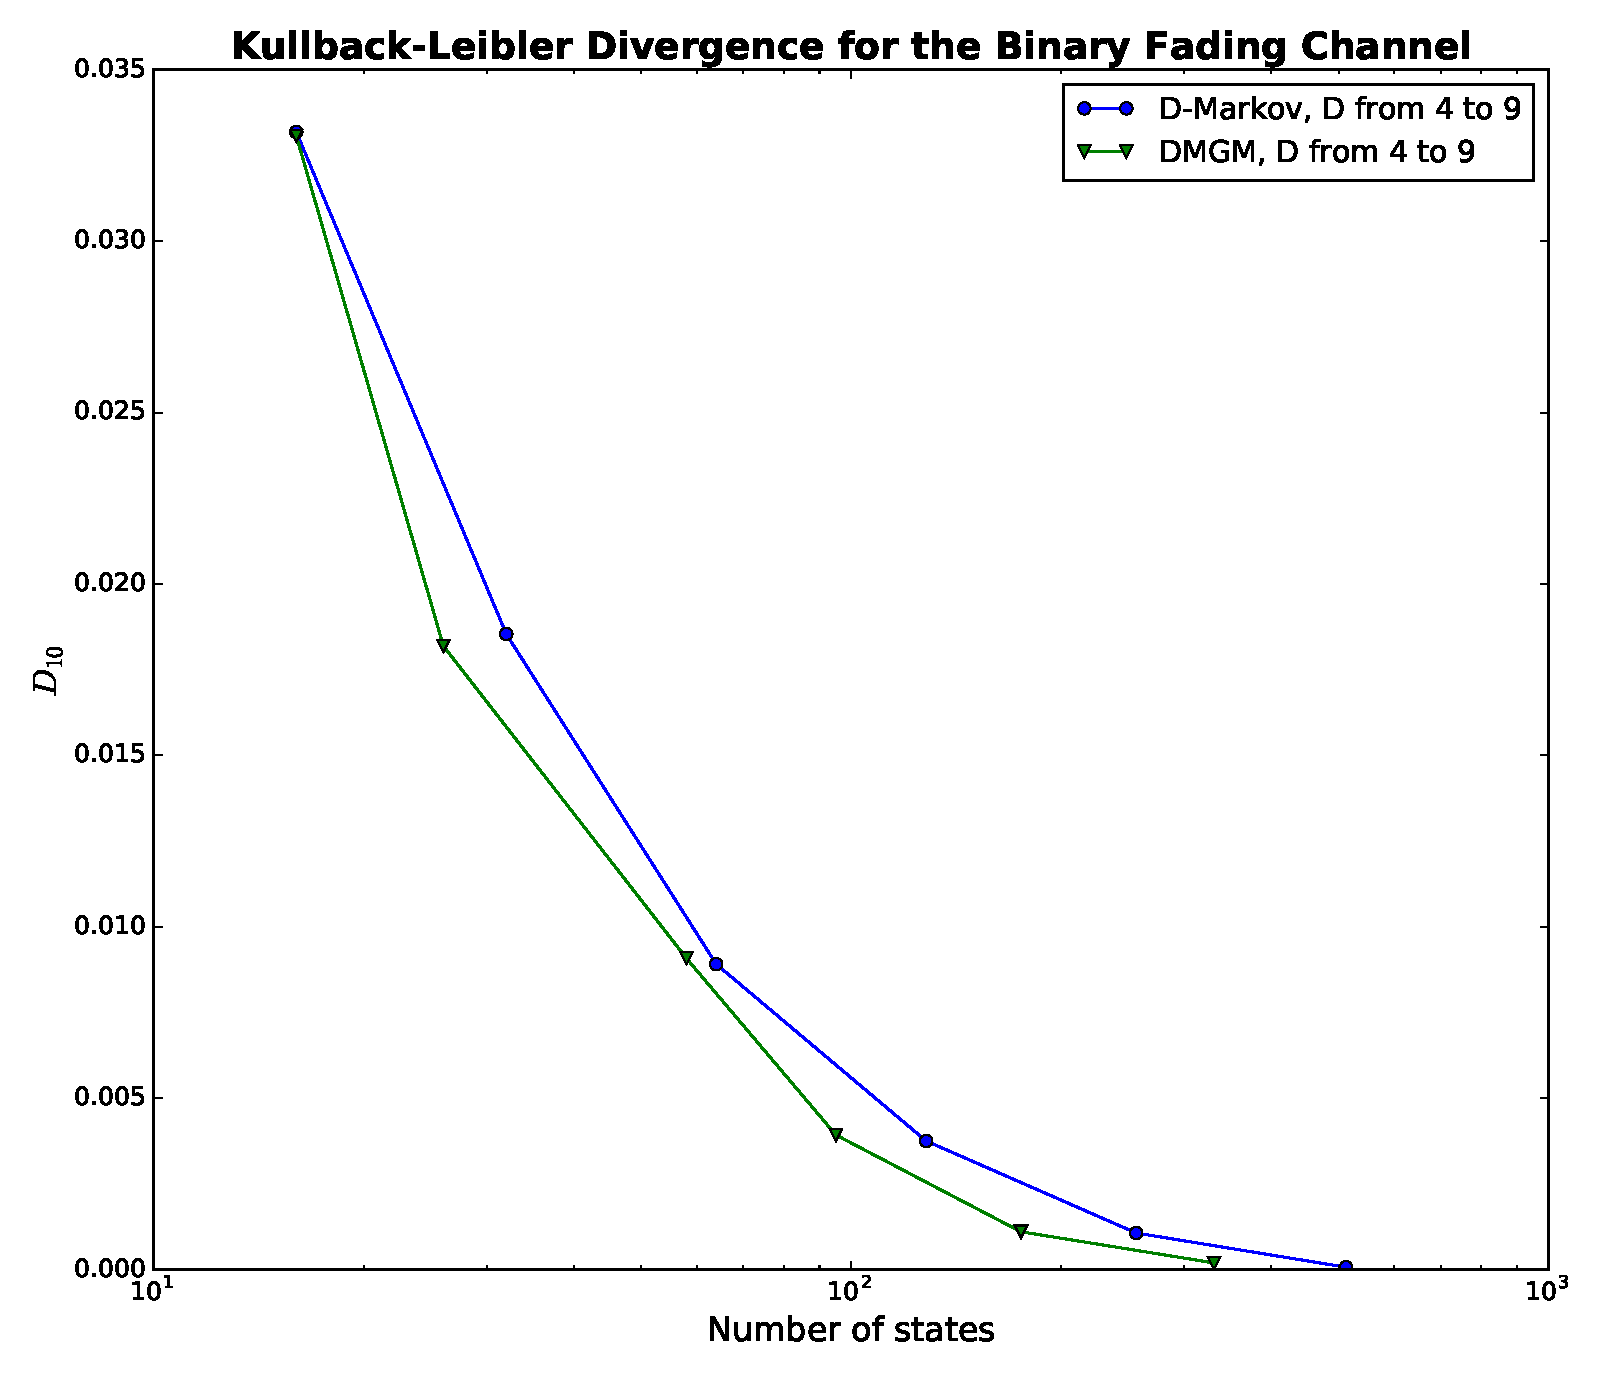
\includegraphics[scale=0.35]{Figuras/10dbq1_kld_mk4.eps}
\caption{Kullback-Leibler divergence $D_{10}$ of sequences generated by D-Markov machines and DMGM PFSA by the number of states of the machine that generated them, with $D$ ranging from 2 to 10, $H=1$ and $t=1$ for the binary fading channel with $f_DT = 0.05$ and $SNR = 10$dB.\label{fig:10dbq1kld}}
\end{figure}

\pagebreak



%From this ternary sequence, the three algorithms were applied in order to obtain a Markovian model for the logistic map. As seen in Table \ref{tab:lmapsynch}, two sets of synchronization words were found for the sequence, one for each of the confidence levels used in the algorithm. For $\alpha = 0.95$, the synchronization words are 2, 00, 01, 10 and 11. On the other hand, for $\alpha = 0.99$, the synchronization words are 2, 00, 01, 10 and 111. The higher value of $\alpha$ made 11 be discarded as synchronization word candidate and allowed 111 to be tested. With the lower value, 11 was never discarded and 111 could not achieve candidate status.
%
%\begin{table}
%\centering
%\caption{Synchronization Words for the Logistic Map Ternary Sequence. \label{tab:lmapsynch}}
%\begin{tabular}{|l|c|c|}
%\hline
% & \multicolumn{2}{c|}{\textbf{$\alpha$}}\\
% \hline
%\textbf{W} & 0.95 & 0.99 \\
%\hline
%2 & 2 & 2 \\ 
%3 & 2, 00, 01, 10, 11 & 2, 00, 01, 10 \\ 
%4 & 2, 00, 01, 10, 11 & 2, 00, 01, 10, 111 \\ 
%5 & 2, 00, 01, 10, 11 & 2, 00, 01, 10, 111 \\
%6 & 2, 00, 01, 10, 11 & 2, 00, 01, 10, 111 \\ 
%7 & 2, 00, 01, 10, 11 & 2, 00, 01, 10, 111 \\ 
% \hline
%\end{tabular}
%\end{table}

%\subsection{Gilbert-Elliot Channel}
%
%The Gilbert-Elliot Channel (GEC) is used to model digital communication channels that suffer with burst errors, i.e. a channel that usually has low probability of error but that has moments where many sequential errors occur. As described in \cite{mushkin.89}, Figure \ref{fig:gec} is the GEC model. It operates in two states, \textit{0} (the "good channel") and \textit{1} (the "bad channel"). While it is in \textit{0}, it works as a Binary Symmetric Channel (BSC) with error probability of $p_0$, which is usually very small, indicating a state in which the channel does not produce too many errors. When it is in state \textit{1}, it is a BSC with error probability $p_1$ which is higher than $p_0$, indicating a state where it is more probable for an error to occur. When in state \textit{0}, it has a probability $q$ of transitioning to state \textit{1} and $1-q$ to stay in \textit{0}. Similarly, when in \textit{1}, it transitions to \textit{0} with probability $q$ and stays with probability $1-q$. This indicates that there is a chance from going to one situation to the other.
%
%\begin{figure}
%\centering
%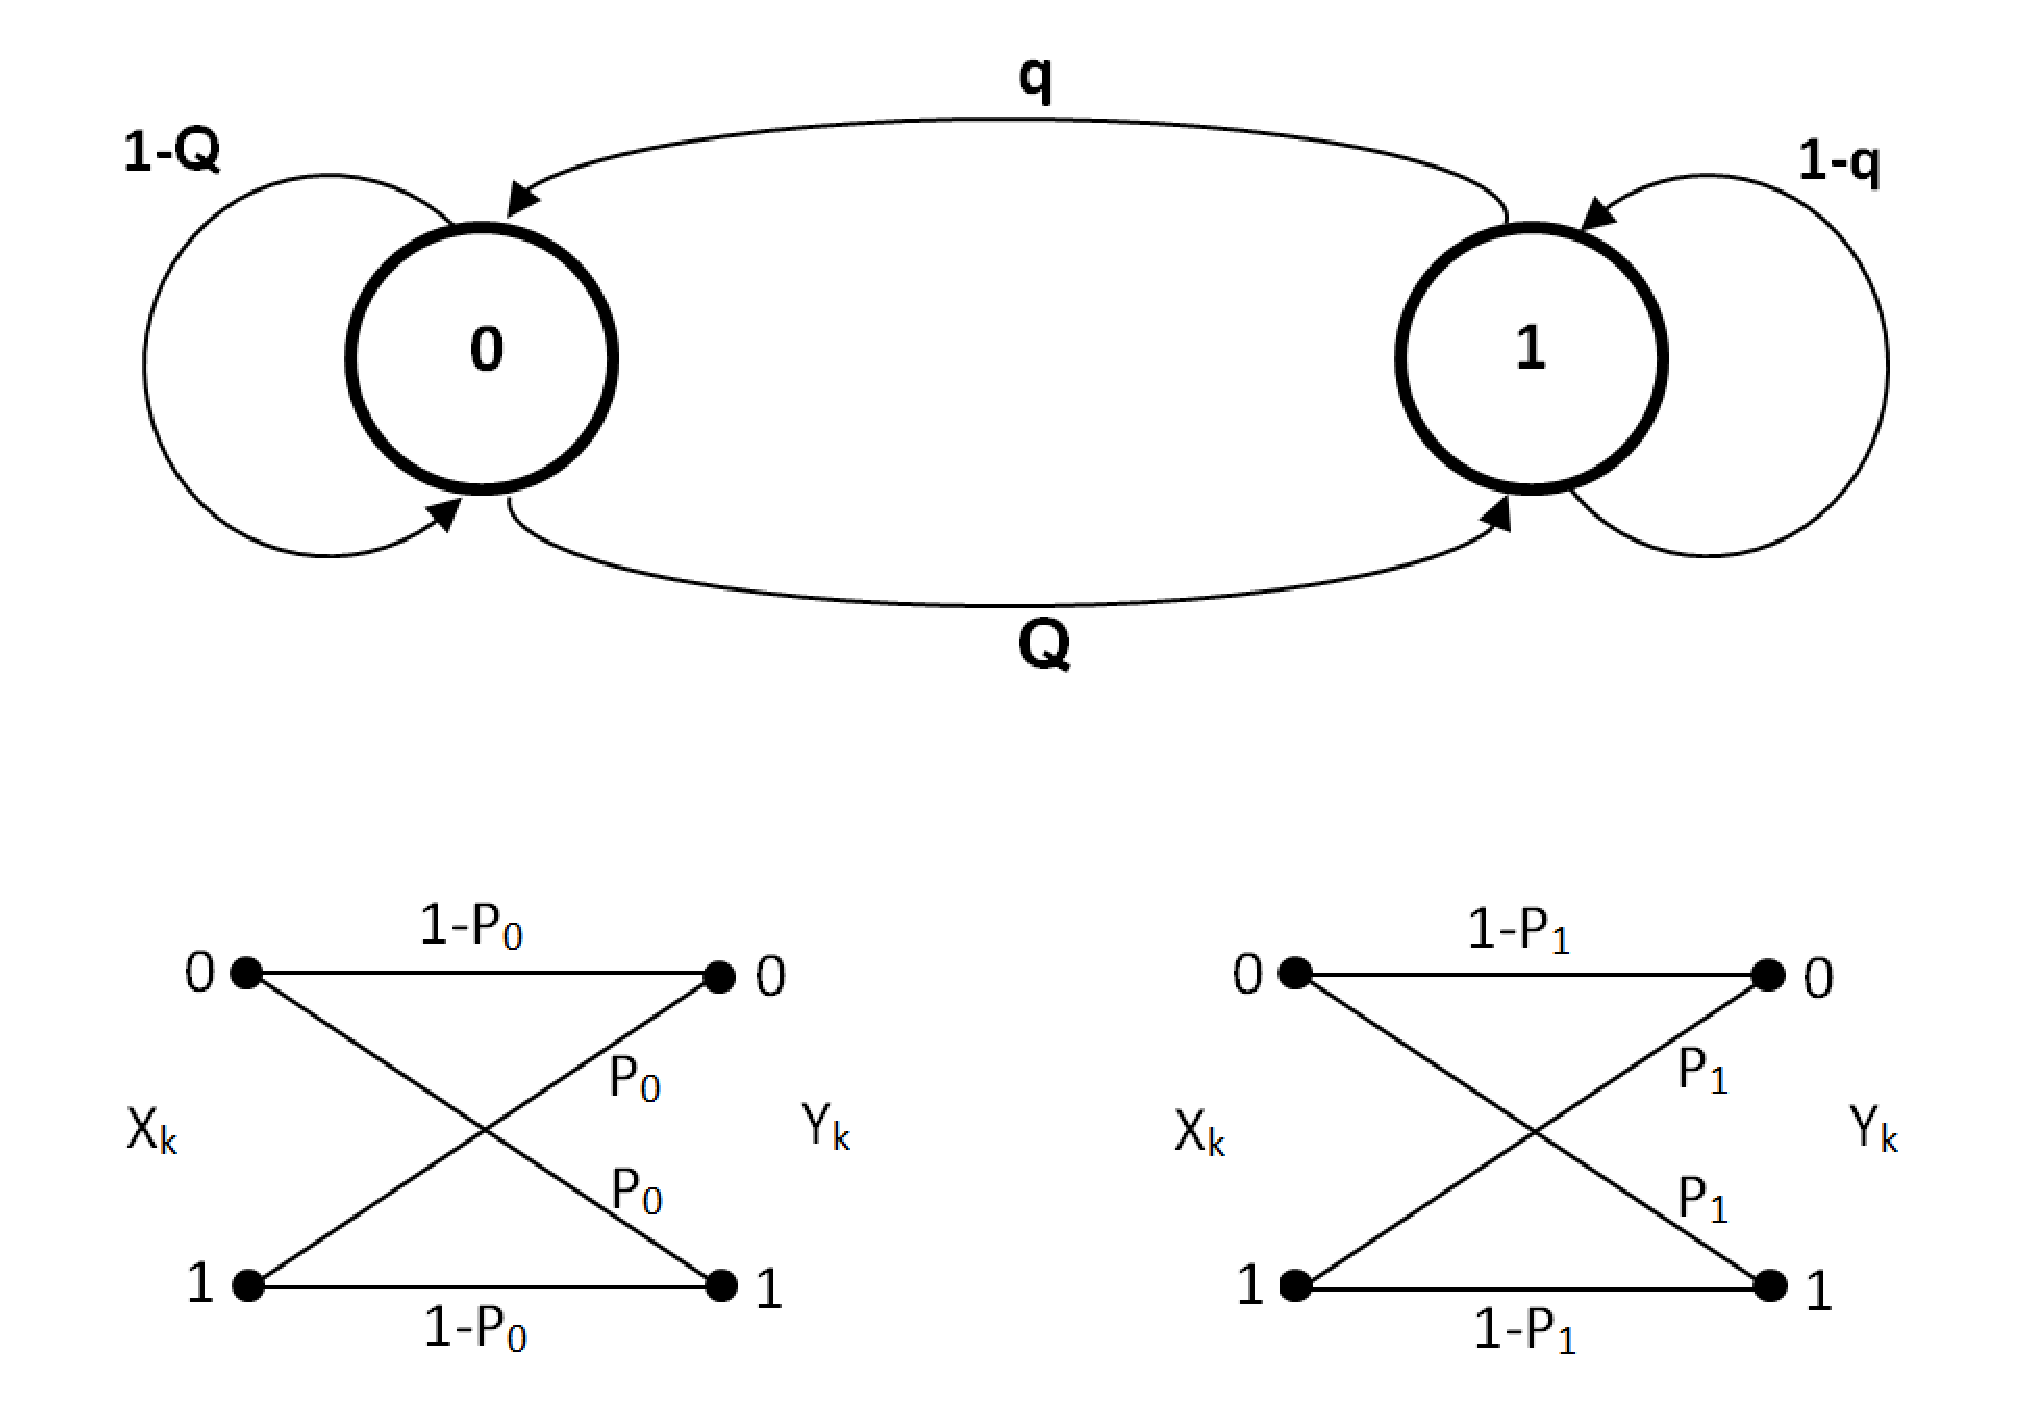
\includegraphics[width=8cm, height=6cm]{Figuras/figgec.eps}
%\caption{\label{fig:gec} The Gilbert-Elliott Channel.}
%\end{figure}
%
%Other important parameters of the GEC that need to be evaluated are its memory $\mu$ and the Bit Error Rate (BER), which is a percentage of errors in the transmission. The memory $\mu$ is defined as:
%
%\begin{equation}
%\mu = 1 - q - Q. \label{eq:mumemory}
%\end{equation}
%
%\noindent which reduces to a memoryless BSC when $\mu = 0$. This parameter is called memory because, as seen in \cite{mushkin.89}, the GEC's autocorrelation function is:
%
%\begin{equation}
%R_{GEC}[m] = (\text{BER})^2 +\frac{Qq(p_1-p_0)²}{(q+Q)²}(1-q-Q)^m, \label{eq:rgec}
%\end{equation}
%
%\noindent which, without getting into much detail, shows that $\mu$ influences how a symbol is related to another one that is $m$ symbols apart. The BER is given by:
%
%\begin{equation}
%\text{BER} = \frac{q}{q+Q}p_0 + \frac{Q}{q+Q}p_1. \label{eq:gecber}
%\end{equation}
%
%The GEC can be designed to obtain specific values of $\mu$ and BER and then it is possible to compare how close to the design parameters the generated PFSA are able to get in order to evaluate their performance.
%
%A binary sequence going through this channel would be output in instant $k$ the following way:
%
%\begin{equation}
%y_k = x_k\oplus z_k, \label{eq:binarychannel}
%\end{equation}
%
%
%\noindent in which $x_k$ is the input symbol at instant $k$, $z_k$ is the error symbol at instant $k$ and $\oplus$ is binary addition operation. When $z_k$ is 0, $y_k$ will be equal to $x_k$, which means that no error occurred. On the other hand, when it 1, $y_k$ will be $x_k \oplus 1 = \neg x_k$, indicating the occurrence of an error. The symbol $z_k$ has a probability $p_e$ of being 1 and $1-p_e$ of being 0 and $p_e$ is equal to $p_0$ if the channel is in state \textit{0} and equal to $p_1$ when it is in state \textit{1}. Following this rule, an error sequence $z$ can be generated to model how the channel and how it affects an input sequence. An error sequence of length $10^{7}$ is generated and used as input to the algorithms. The GEC is strictly not Markovian and this is an example to show how the algorithms fare in modeling such a system in a Markovian fashion.